\documentclass[10pt]{beamer}

\usetheme[progressbar=frametitle]{metropolis}
\usepackage{appendixnumberbeamer}

\usepackage{booktabs}
\usepackage[scale=2]{ccicons}

\usepackage{pgfplots}
\usepgfplotslibrary{dateplot}

\usepackage{xspace}
\newcommand{\themename}{\textbf{\textsc{metropolis}}\xspace}

\title{
    Verification of Recoil Separator Properties Through Reaction Measurements
}
\subtitle{}
% \date{\today}
\date{November 9, 2018}
\author{Michael T Moran}
\institute{University of Notre Dame}
% \titlegraphic{\hfill\includegraphics[height=1.5cm]{logo.pdf}}

\begin{document}

\maketitle

\begin{frame}{Table of contents}
  \setbeamertemplate{section in toc}[sections numbered]
  \tableofcontents[hideallsubsections]
\end{frame}

\section{Introduction}

\begin{frame}[fragile]{Nuclear Astrophysics}

    Placeholder

\end{frame}

\begin{frame}[fragile]{Radiative Capture}

    Placeholder

\end{frame}

\section{Recoil Separation}

\begin{frame}{Particle Selection}
    We can uniquely identify particles by their mass, charge and energy:

    \begin{alertblock}{Magnetic Selection}
        \[
            \frac{m}{q} = \frac{B\rho}{2}\left(\frac{T}{q}\right)^{-1}
        \]
    \end{alertblock}
    \begin{alertblock}{Electric Selection}
        \[
            \frac{T}{q} = \frac{E\rho}{2}
        \]
    \end{alertblock}
    \begin{alertblock}{Wien Filter Selection}
        \[
            \frac{m}{q} = \frac{2}{v^2} \frac{T}{q}
        \]
    \end{alertblock}

\end{frame}

\begin{frame}{Particle Selection}

    Any two of the three possibilities may be combined to uniquely
    identify a particle

    \begin{figure}
        \includegraphics[width=0.75\textwidth]%
            {figures/particle_selection_by_field.png}
    \end{figure}

\end{frame}

\begin{frame}{St.\ George}

    \begin{figure}
        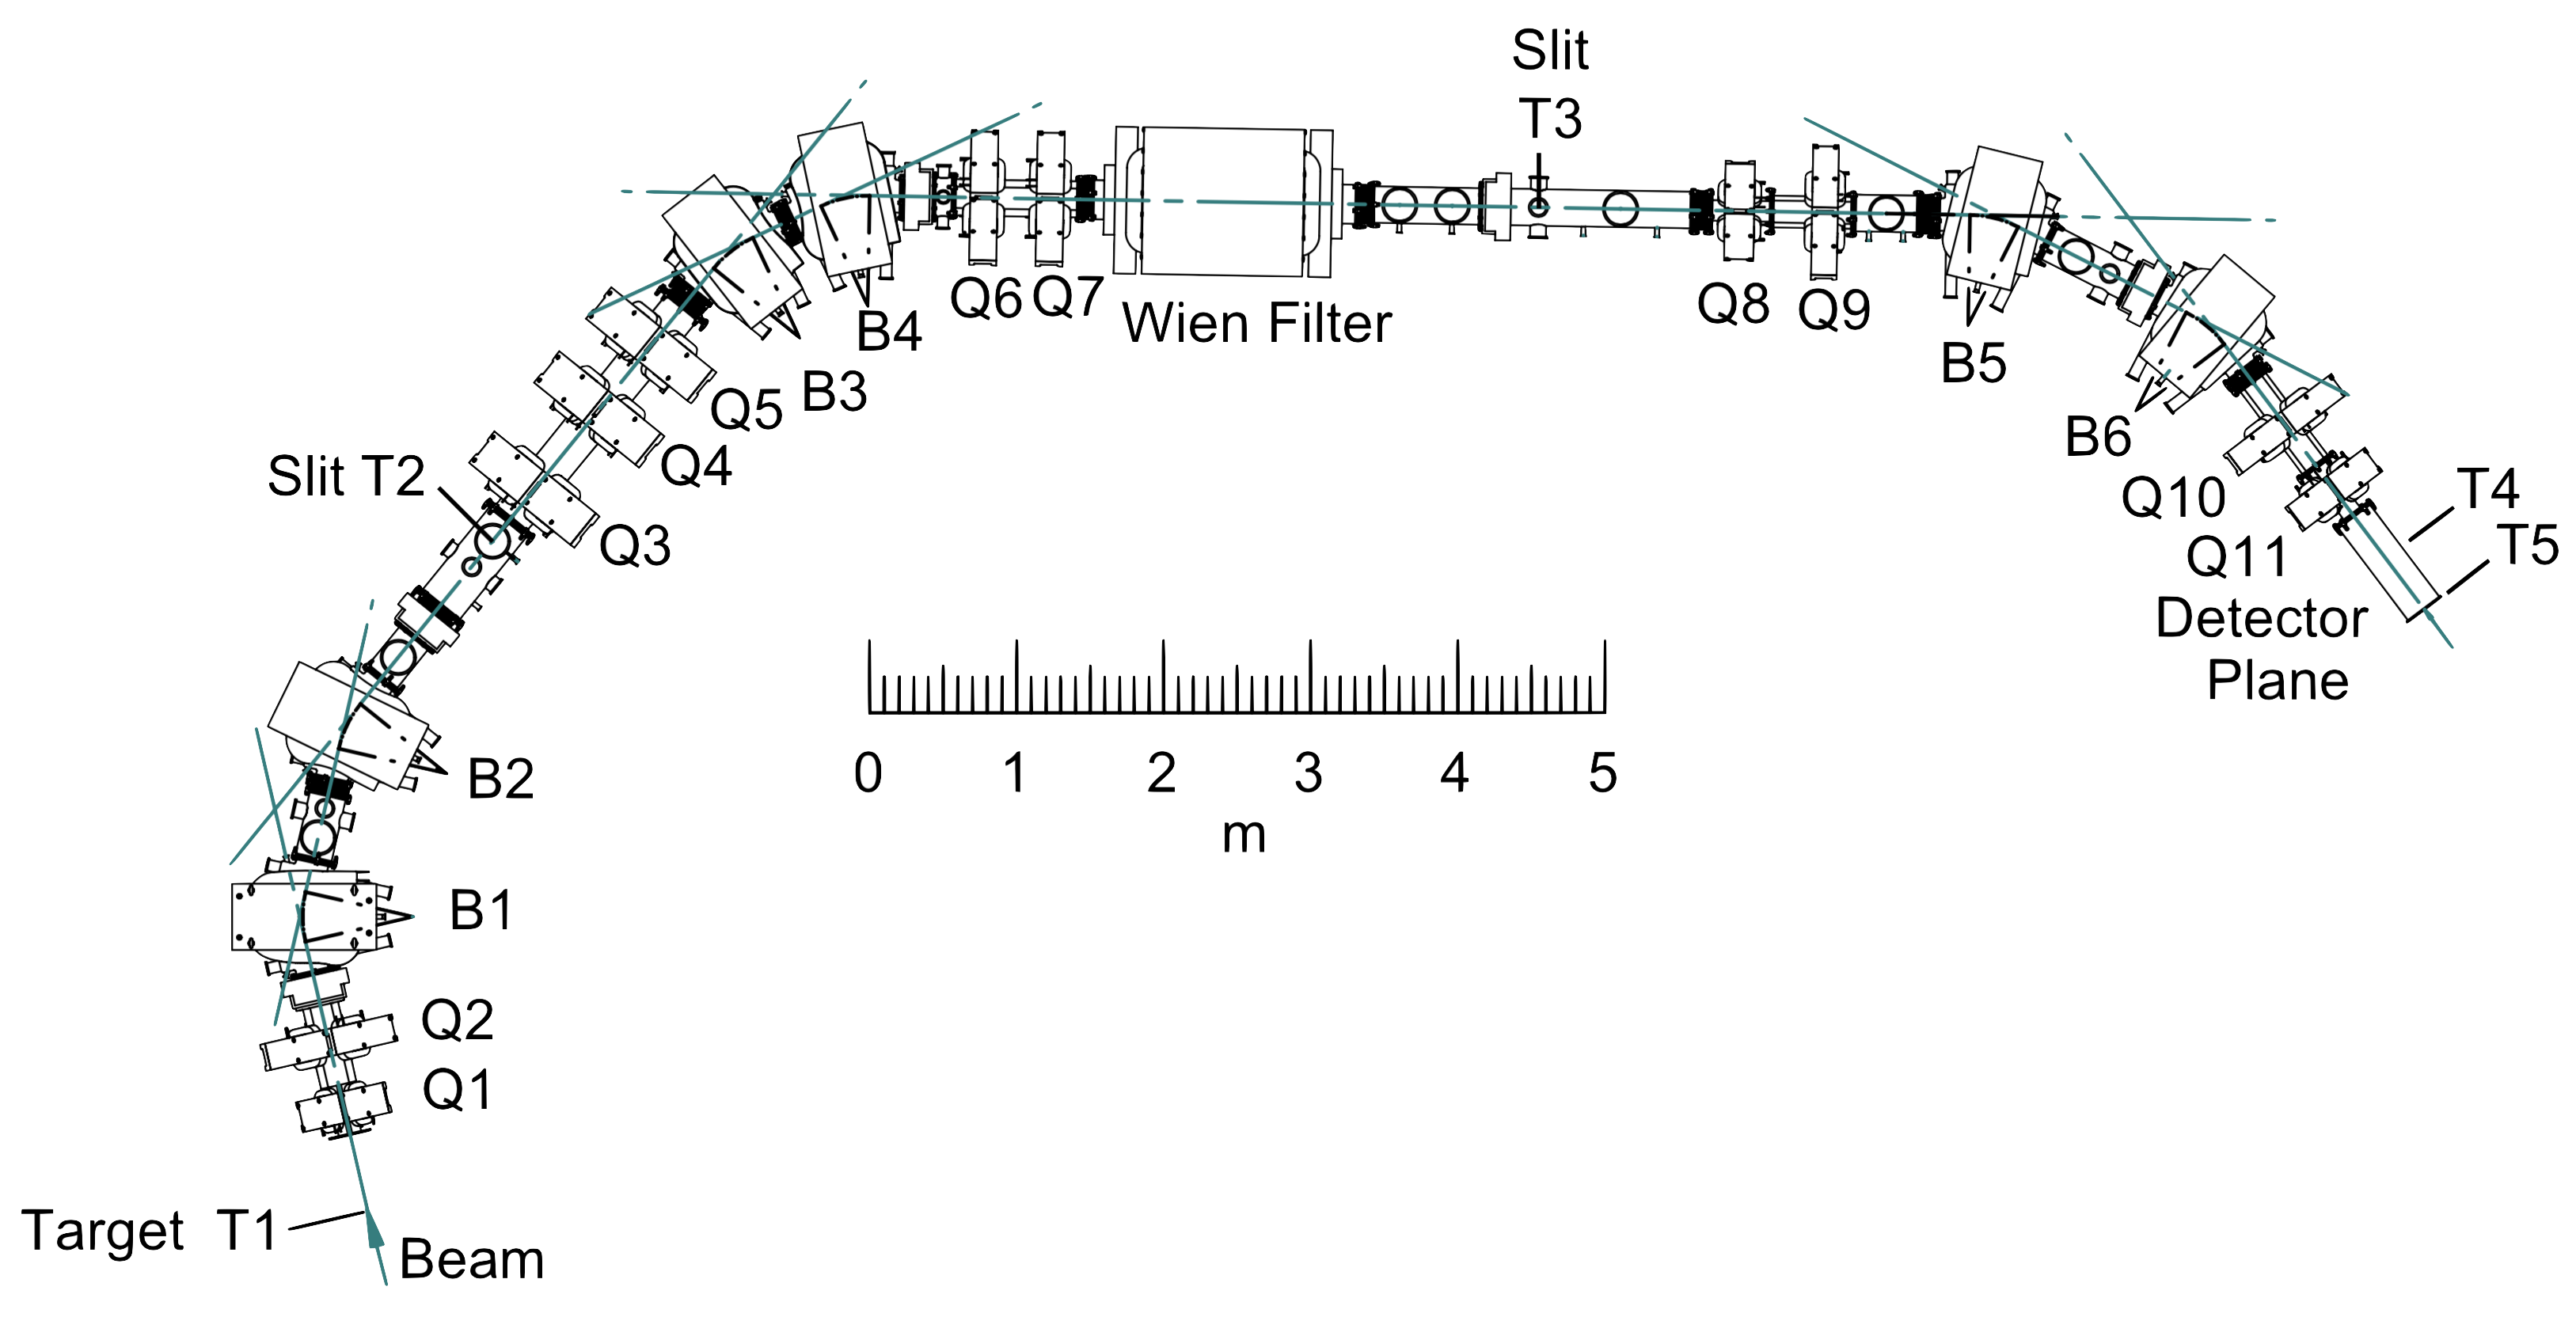
\includegraphics[width=0.95\textwidth]{figures/stg.png}
    \end{figure}

\end{frame}

\appendix

\begin{frame}[fragile]{Backup slides}

\end{frame}

\begin{frame}[allowframebreaks]{References}

  \bibliography{defense}
  \bibliographystyle{abbrv}

\end{frame}

\end{document}
